%-------------------------------------------------------------------------------------------------------
%-------------------------------------------------------------------------------------------------------
%-------------------------------------------------------------------------------------------------------
\subsection{Introducci\'on a la secci\'on}
Cada apartado es una simulaci\'on de la futura aplicaci\'on del algoritmo. Cada una consta de una escena propia mostrada como en la figura \ref{fig:VREP_scene_example}. El resultado se visualiza por consola en el formato que muestra la figura \ref{fig:Ground_Tracking_VREP_Console}. \\

\begin{figure}[ht]
	\centering
	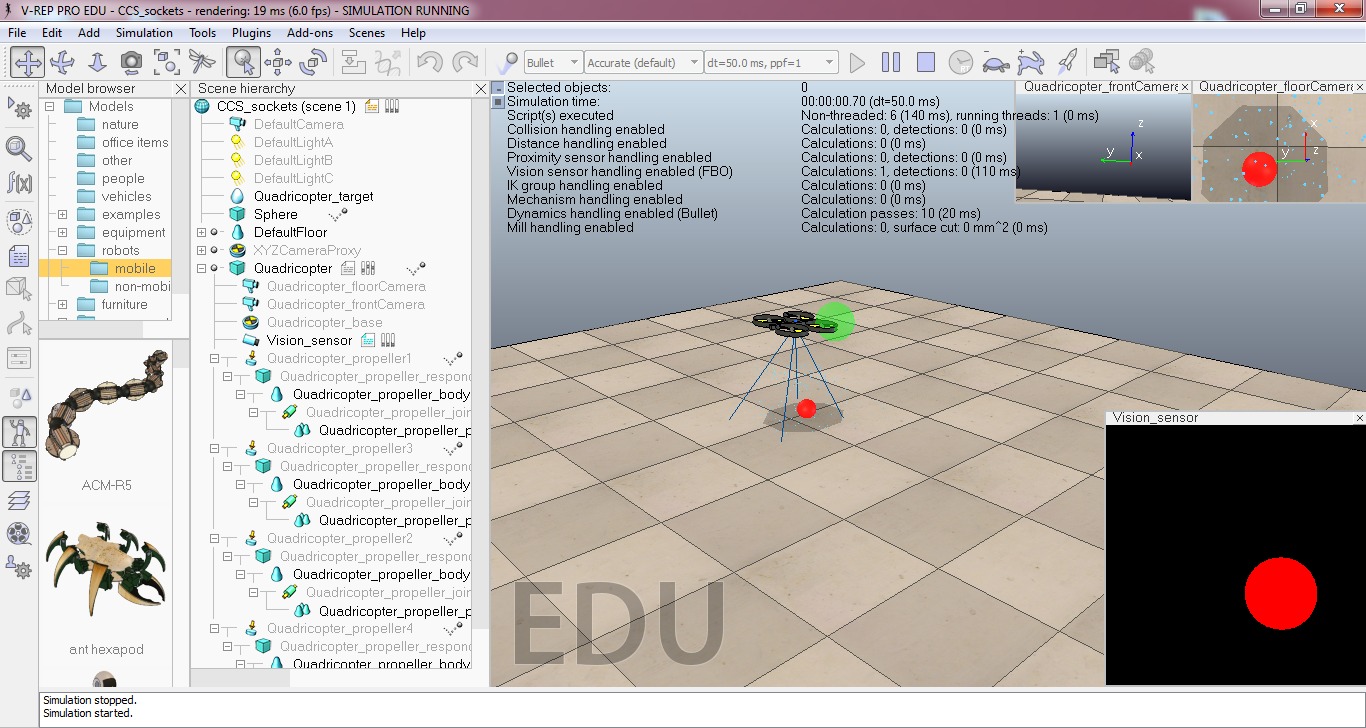
\includegraphics[width=0.8\textwidth,natwidth=1366,natheight=728]{../Images/c3/ground_tracking_scene.png}
	\caption{Ground Tracking Scene}
	\label{fig:VREP_scene_example}
\end{figure}

\begin{figure}[ht]
	\centering
	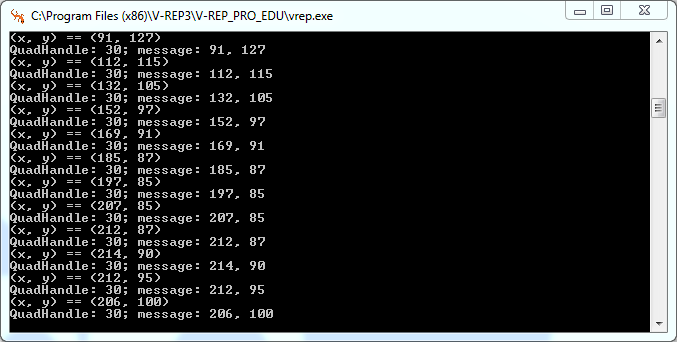
\includegraphics[width=0.8\textwidth,natwidth=677,natheight=342]{../Images/c3/ground_tracking_vrep_console.png}
	\caption{Ground Tracking V-REP Console}
	\label{fig:Ground_Tracking_VREP_Console}
\end{figure}

La estación en tierra se simula con una aplicaci\'on en el mismo ordenador que ejecuta la simualaci\'on tal que los resultados se muestran tambi\'en por consola del siguiente modo: \ref{fig:Ground_Tracking_Server_Console}.

\begin{figure}[ht]
	\centering
	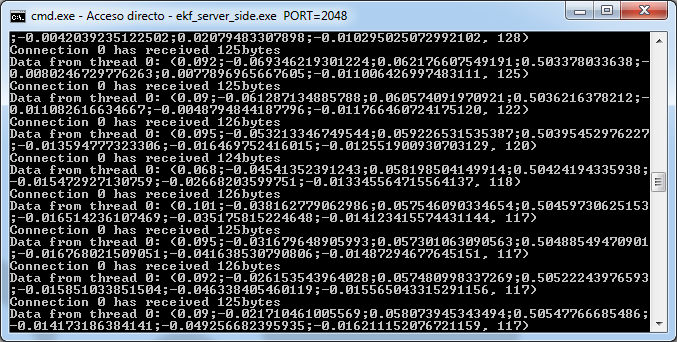
\includegraphics[width=0.8\textwidth,natwidth=677,natheight=342]{../Images/c3/ground_tracking_server_console.png}
	\caption{Ground Tracking Server Console}
	\label{fig:Ground_Tracking_Server_Console}
\end{figure}

Ambos procesos (Quadrotor y estaci\'on de tierra) generan unos ficheros de LOG que se usar\'an para analizar los resultados.

%-------------------------------------------------------------------------------------------------------
%-------------------------------------------------------------------------------------------------------
%-------------------------------------------------------------------------------------------------------
%-------------------------------------------------------------------------------------------------------
%-------------------------------------------------------------------------------------------------------
%-------------------------------------------------------------------------------------------------------
\subsection{Ejemplo de resultados - Seguimiento en tierra de m\'ultiples objetivos}
\subsubsection{Preparaci\'on}
 Este experimento consta de un solo quadrotor y dos obetivos \ref{fig:sim4_set_up}.
 
\begin{figure}[htp]
	\centering
	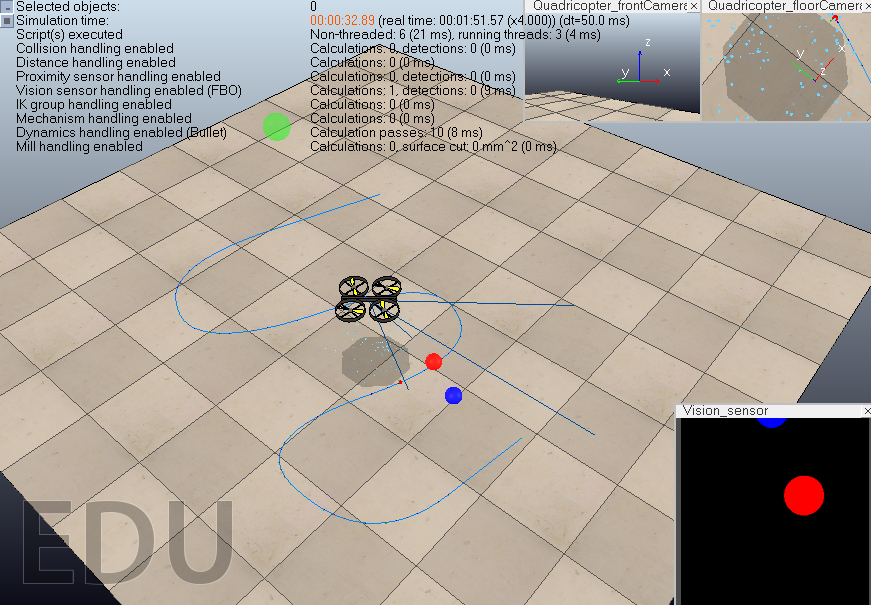
\includegraphics[width=0.4\linewidth]{../Images/c3/sim4_set_up}
	\caption{Objetivos M\'ultiples objetivos}
	\label{fig:sim4_set_up}
\end{figure}

\subsubsection{Test y resultados}

	Como en los apartados anteriores se muestran tres figuras correspondientes a las coordenadas XY original y calculada y la trayectoria 3D (\ref{fig:sim4_redtarget}, \ref{fig:sim4_bluetarget} y \ref{fig:sim4_3dtraj}). \\
	
	\begin{figure}[hp]
		\centering
		\begin{subfigure}[hp]{0.45\linewidth}
			\centering
			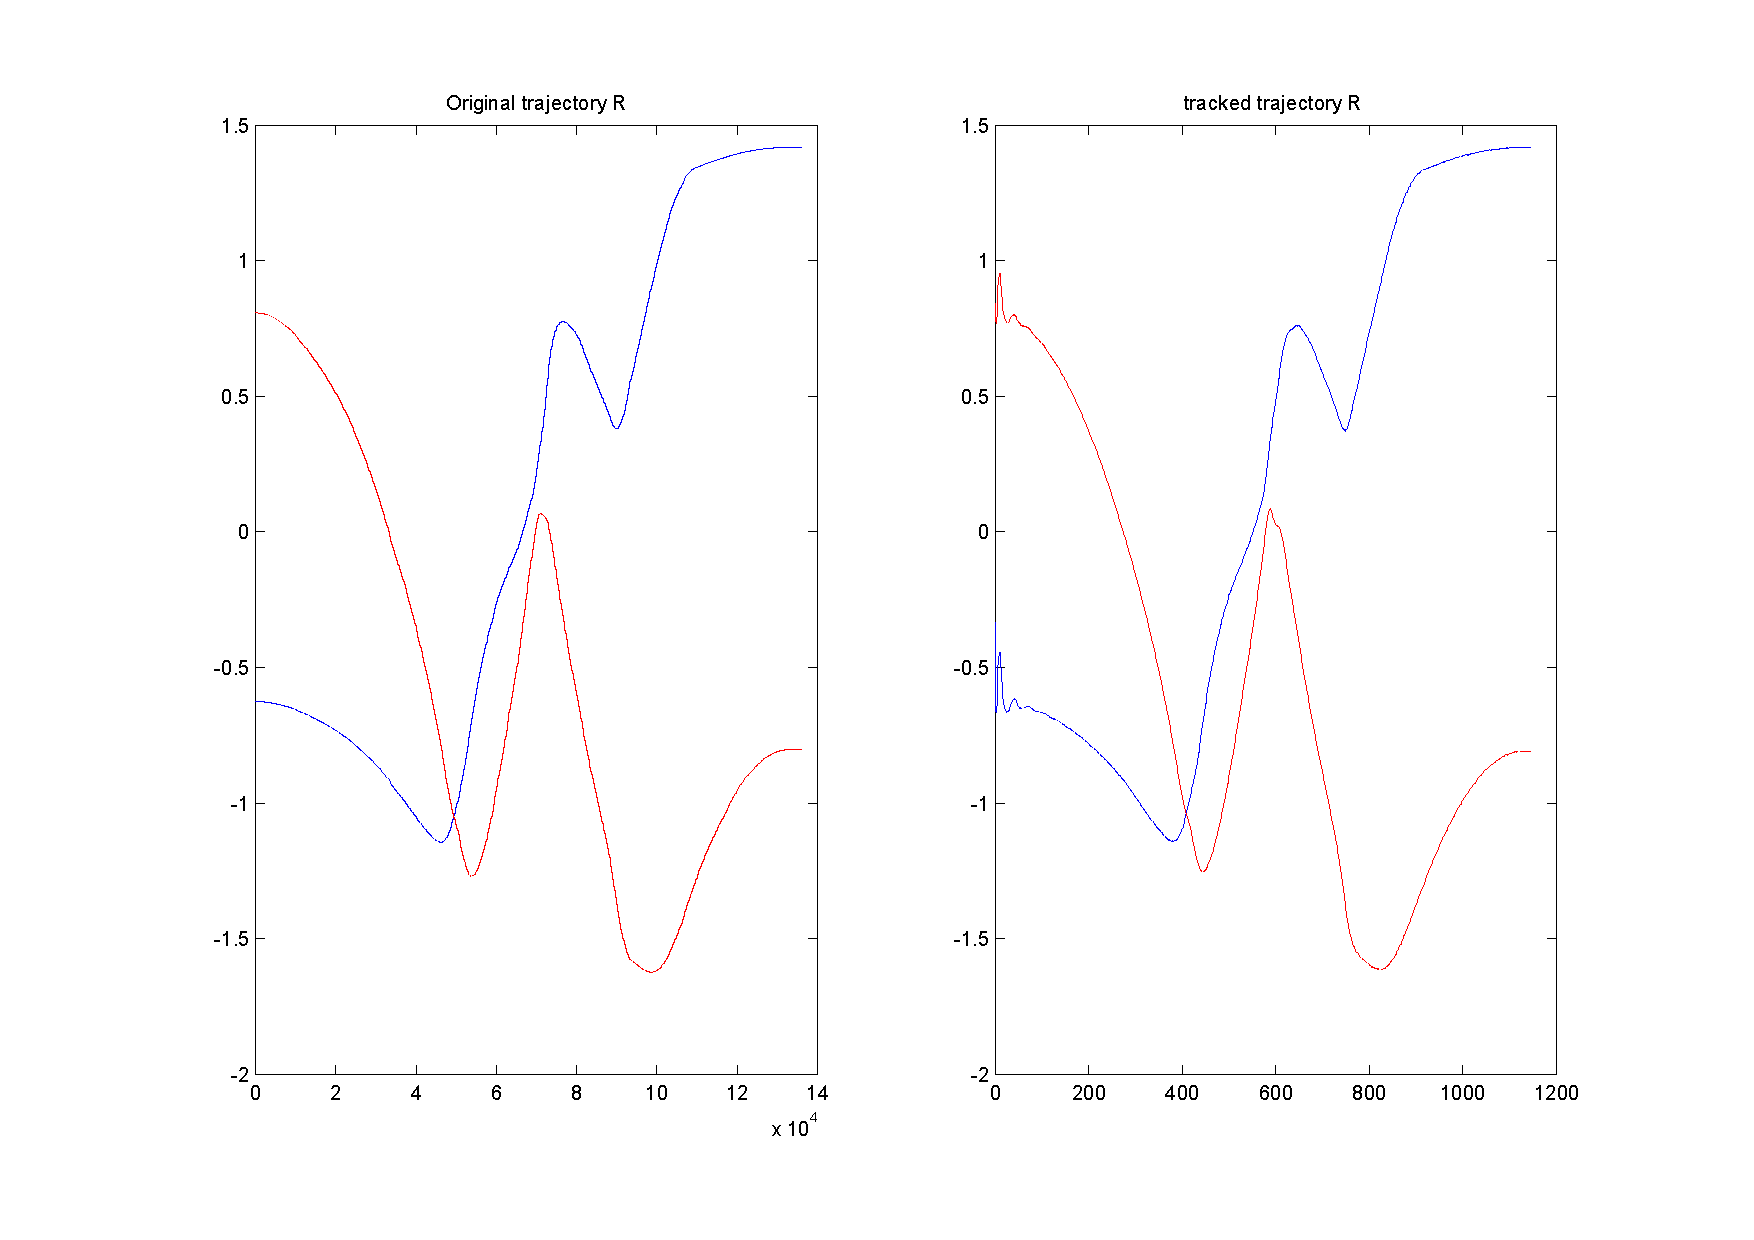
\includegraphics[width=\linewidth]{../Images/c3/sim4_redtarget}
			\caption{Multiple Targets - Red target}
			\label{fig:sim4_redtarget}	
		\end{subfigure}
		~
		\begin{subfigure}[hp]{0.45\linewidth}
			\centering
			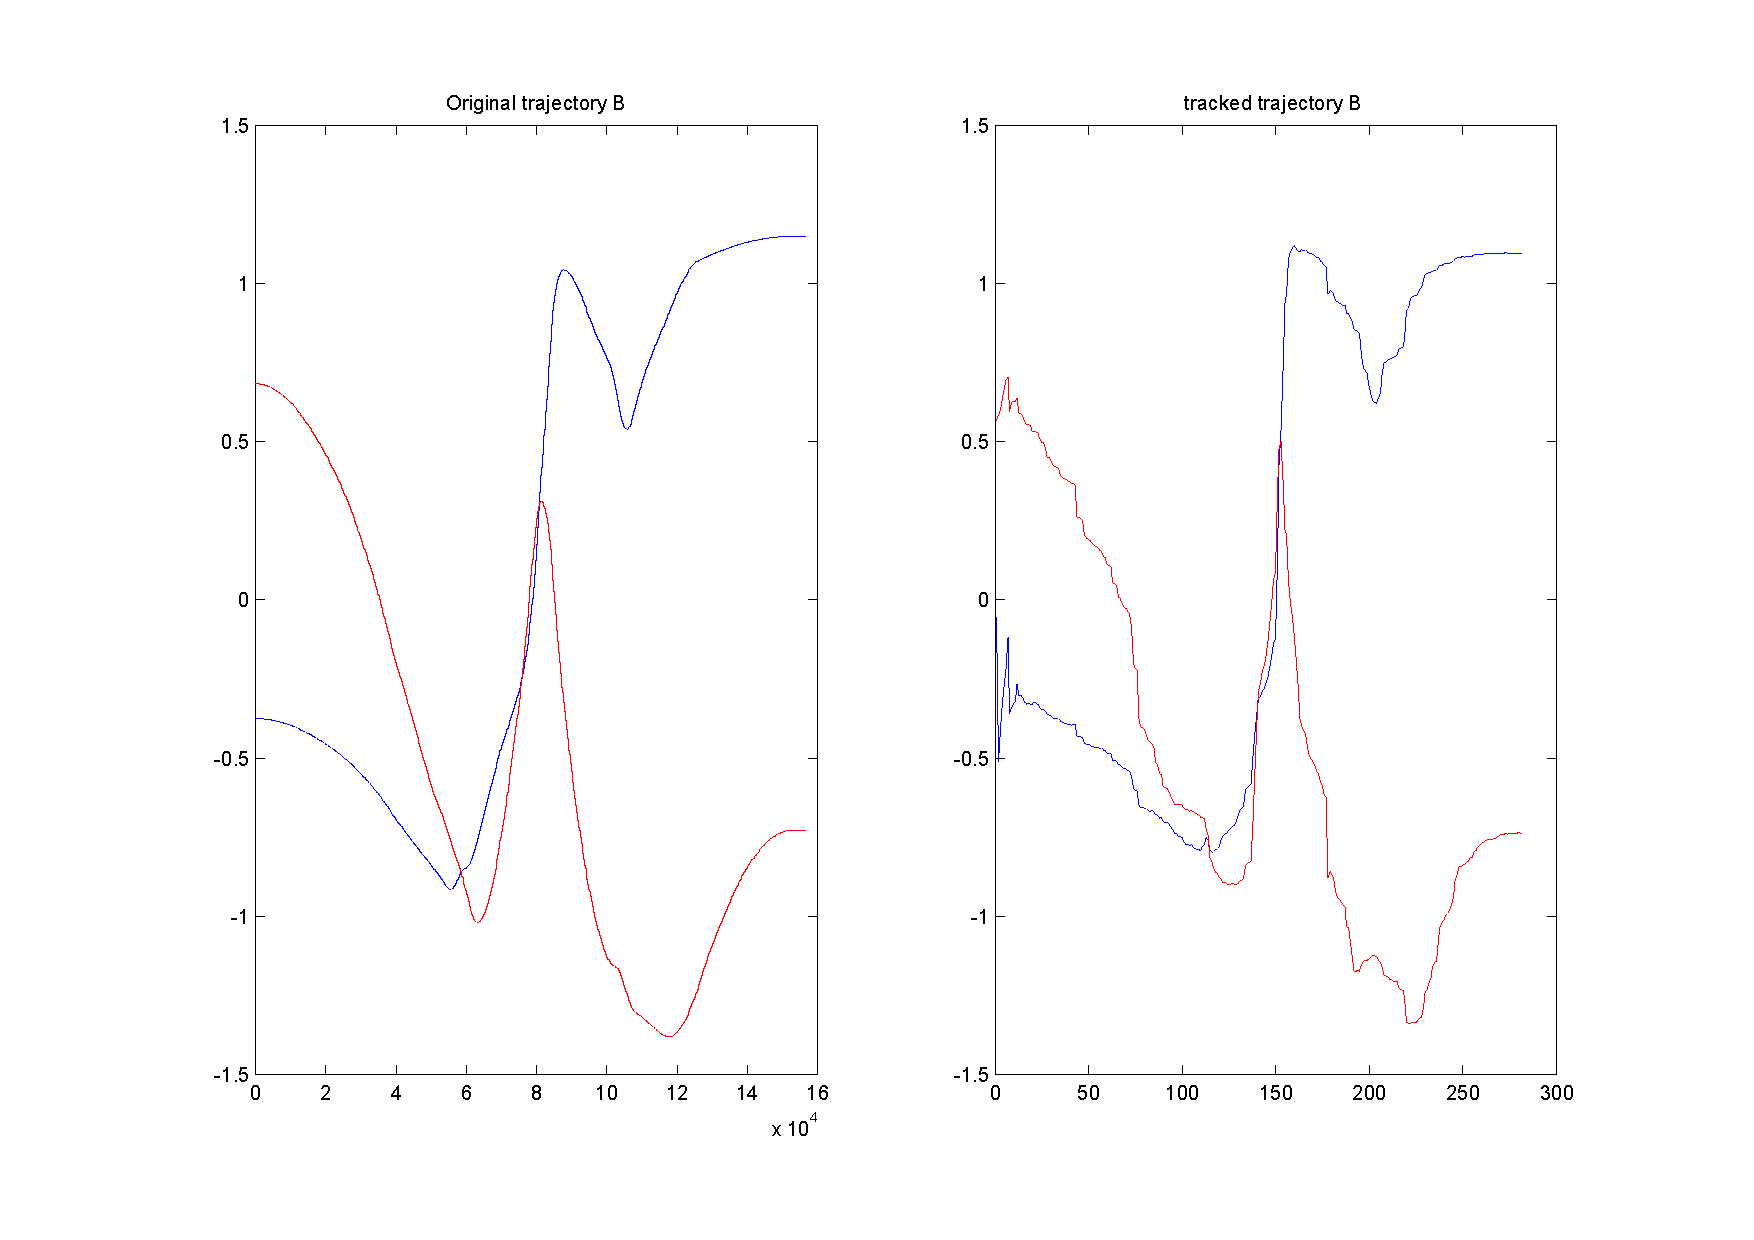
\includegraphics[width=\linewidth]{../Images/c3/sim4_bluetarget}
			\caption{Multiple Targets - Blue target}
			\label{fig:sim4_bluetarget}
		\end{subfigure}
	\end{figure}
	
	Los resultados esta simulaci\'on son buenos igual que en los apartados anteriores \ref{fig:sim2_traj_both_3d}. El resultado del seguimiento del objeto azul puede parecer erroneo inicialmente, sin embargo es un resultado totalmente coherente ya que este nunca se ve completamente por lo que nunca se obtiene el centro real del mismo \ref{fig:sim4_centroid_objs} y de ah\'i el error en posici\'on. El error m\'aximo en el azul es $\sim$ 15 cm y el medio es $\sim$ 6 cm.



\begin{figure}[hp]
	\centering
	\begin{subfigure}{0.45\linewidth}
		\centering
		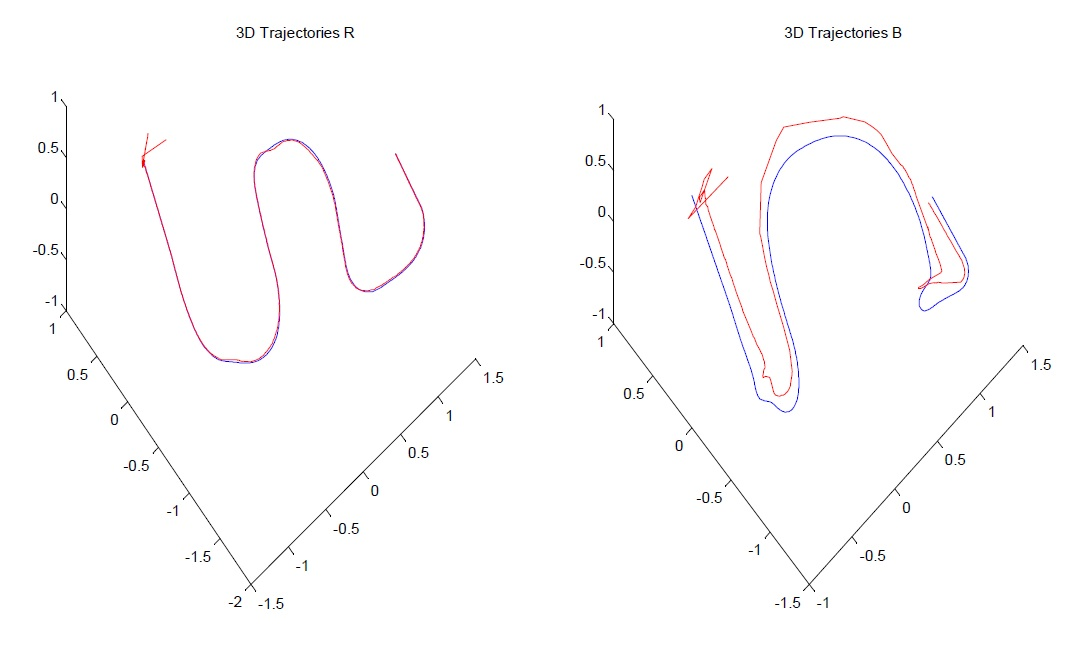
\includegraphics[width=\linewidth]{../Images/c3/sim4_3dtraj}
		\caption{M\'ultiples objetivos - Trayectoria 3D}
		\label{fig:sim4_3dtraj}
	\end{subfigure}
	~
	\begin{subfigure}{0.2\linewidth}
		\centering
		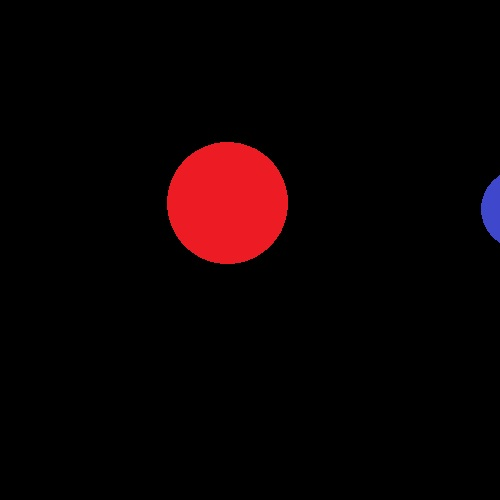
\includegraphics[width=\linewidth]{../Images/c3/sims_two_object_centroid_out}
		\caption{M\'ultiples objetivos - Centroides}
		\label{fig:sim4_centroid_objs}
	\end{subfigure}
\end{figure}